\documentclass[proposal.tex]{subfiles}



\begin{document}


% ---------------------------------------------------------------------------
\chapter{Related Concepts}\label{chap:relatedWork}
% ---------------------------------------------------------------------------


\section{About this chapter}

\noindent\rule{\textwidth}{0.5pt}
%-----------------------------------------------------------------------------


\section{Warren abstract machine}
There are some technicalities which are indirectly related to the problem but do not bare a point of contact.
The underpinnings of the languages throw some more light on the how different languages work to solve a problem.
Different programming paradigms incorporate different operational mechanisms.
For example, \progLang{Prolog} programs execute on the Warren Abstract Machine \cite{ait1999warren} which has three
different storage usages; a global stack for compound terms, for environment frames and choice points and lastly
the trail to record which variables bindings ought to be undone on backtracking.

\section{Constraint programming}
Constraint programming \cite{website:constraintprogwiki} is closely related to the declarative programming paradigm
in the sense that the relations between variables is specified in the form of constraints.
For example, consider a program to solve a simultaneous equation, now adding on to that restricting the range of
the values that the variables can possible take, thus adding constraints to the possible solutions.
Related to the same are constraint handling rules \cite{website:chrwiki}, which are extensions to a language,
simply speaking adding constraints to a language like \progLang{Prolog}.


\section{Residuation and narrowing}
Lastly some details on the working of functional logic programming languages, residuation and narrowing
\cite{hanus1995curry,webiste:wikicurry}.
Residuation involves delaying of functions calls until they are deterministic, that is, deterministic reduction of
functions with partial data.
This principle is used in languages like \progLang{Escher} \cite{lloyd1999programming:escher}, \progLang{Life}
\cite{website:life}, \progLang{NUE-Prolog} \cite{website:nue-prolog} and \progLang{Oz} \cite{website:oz-mozart}.
Narrowing on the other hand is a mixture of reduction in functional languages and unification in logic languages.
In narrowing, a variable is bound a value within the specified constraints and try to find a solution, values are
generated while searching rather than just for testing.
The languages based on this approach are \progLang{ALF} \cite{website:alf}, \progLang{Babel} \cite{website:babel},
\progLang{LPG} \cite{bert1987lpg} and \progLang{Curry} \cite{website:curry}.


\section{F-Algebras}


We are now ready to define \markWord{F}-algebras in the most general terms.
First I'll use the language of category theory and then quickly translate it to \progLang{Haskell}.

An \markWord{F}-algebra consists of:
\begin{enumerate}
\item an endofunctor \markWord{F} in a category \markWord{C},
\item an object \markWord{A} in that category, and
\item a morphism from \markWord{F(A)} to \markWord{A}.
\end{enumerate}

An \markWord{F}-algebra in \progLang{Haskell} is defined by a functor \haskellConstruct{f}, a carrier type \markWord{a}, and a function from \markWord{(f a)} to \markWord{a}. (The underlying category is \haskellConstruct{Hask}.)

Right about now the definition with which I started this post should start making sense:

\mint{haskell}|type Algebra f a = f a -> a|

For a given functor \haskellConstruct{f} and a carrier type \markWord{a} the algebra is defined by specifying just one function.
Often this function itself is called the algebra, hence my use of the name \markWord{alg} in previous examples.


\section{Monads by example: The State Monad}

In this section we try and replicate a dictionary of variables. The operations such as adding and removing entries to and from the
dictionary are implemented so as to replicate modification. Listing~\ref{tab:hskllmndworkngdatatype} shows the structure of the 
\haskellConstruct{IntegerDictionary} for storing and modifying the \haskellConstruct{Variables}. Each \haskellConstruct{Variable} is a \haskellConstruct{VariableName}, \haskellConstruct{Value} pair.
 
\begin{code-list}[H]
  \begin{singlespace}
    \inputminted[linenos, firstline=22, lastline=33]{haskell}{haskell-monad-working-2.hs}
  \end{singlespace}
  \caption{Haskell Monad Working: Data Types}
\label{tab:hskllmndworkngdatatype}
\end{code-list}

Listing~\ref{tab:hskllmndworkngfunctions} shows the insertion and removal in a variable dictionary and the \haskellConstruct{run} function 
for applying the operation on the dictionary.

\begin{code-list}[H]
  \begin{singlespace}
    \inputminted[linenos, firstline=35, lastline=76]{haskell}{haskell-monad-working-2.hs}
  \end{singlespace}
  \caption{Haskell Monad Working: Functions}
\label{tab:hskllmndworkngfunctions}
\end{code-list}

Listing~\ref{tab:hskllmndworkngexamples} shows a combination of the operation of finding a product of the two variables and 
storing back the result in the dictionary.


\begin{code-list}[H]
  \begin{singlespace}
    \inputminted[linenos, firstline=81, lastline=123]{haskell}{haskell-monad-working-2.hs}
  \end{singlespace}
  \caption{Haskell Monad Working: Examples}
\label{tab:hskllmndworkngexamples}
\end{code-list}


%% dgc : The [] in the section heading avoids having the reference show
%% up in the table of contents.  
\section[{The execution models of \progLang{Prolog}}]{The execution models of \progLang{Prolog} \cite{Sterling:1994:APA:175753}\endnote{
\david{Move the citation from the section title, and explicitly state that
  the material here has been exerpted from
  \cite{Sterling:1994:APA:175753}, with page or chapter references.
}
\mehul{changed}
}
}\label{sec:exec-models-prolog}
Logic programming languages are adapted from abstract interpreters for logic programs. 
To implement a logic programming language such as \progLang{Prolog} two major decisions must be taken to resolve a query\endnote{
\david{Rewrite this to be clear about the differences between an
  \textit{abstract} \progLang{Prolog} and the choices made by concrete
  implementations, such as Edinburgh \progLang{Prolog}.
}
\mehul{changed}
}:
\begin{enumerate}
\item Scheduling policy:
Select leftmost goal and replace the non deterministic choice of a clause by sequential search for a unifiable clause and backtracking. 
Stack scheduling policy, pop the topmost goal for reduction and push derived goals back.

\item Search strategy:
\progLang{Prolog} simulates the non-deterministic choice of reducing clause by sequential search and backtracking. The first goal whose 
head unifies with the goal is chosen. If no match is found then the computation is unwound to the last choice point and the next unifiable 
clause is chosen.
\end{enumerate}

\progLang{Prolog} generates all possible solutions of the goal with respect to the \progLang{Prolog} program. It performs a complete
depth first traversal of a particular search tree for the goal by always choosing the leftmost goal. Listing~\ref{tab:prlgprgrmtrce} shows
a sample trace for a query.

\begin{code-list}[H]
  \begin{singlespace}
    \inputminted[linenos]{prolog}{prologprogramtrace.pl}
  \end{singlespace}
  \caption{Tracing a simple Prolog computation \cite{Sterling:1994:APA:175753}}
\label{tab:prlgprgrmtrce}
\end{code-list}

As seen in Listing~\ref{tab:prlgprgrmtrce} how \progLang{Prolog} resolves a query. Consider the example in 
Listing~\ref{tab:prlgcutfreeexmpl}. A sample query \prologConstruct{p(X)} will result in \ref{tab:prlgcutfreeexmploutput}. 

\begin{code-list}[H]
  \begin{singlespace}
    \inputminted[linenos]{prolog}{prlgcutfreeexmpl.pl}
  \end{singlespace}
  \caption{A cut-free Prolog computation \cite{website:cutprologunionedu}}
\label{tab:prlgcutfreeexmpl}
\end{code-list}

\begin{code-list}[H]
  \begin{singlespace}
    \inputminted[linenos]{prolog}{prlgcutfreeexmploutput.pl}
  \end{singlespace}
  \caption{cut-free Prolog computation output\cite{website:cutprologunionedu}}
\label{tab:prlgcutfreeexmploutput}
\end{code-list}

A \prologConstruct{cut} represented as \prologConstruct{!} operator \cite{website:prologcut}.
If \progLang{Prolog} finds a \prologConstruct{cut} in a rule, it will not backtrack on the choices it has made. Consider the example below:

\mint{prolog}|p(X) :- b(X),c(X),!,d(X),e(X).|

The result for a sample query \prologConstruct{p(X)}:
\mint{prolog}|X = 1 ; no|

Only a single solution is obtained because the \prologConstruct{cut} prevents backtracking. The Figure~\ref{fig:Trace with cut} shows the 
trace for the query with the \prologConstruct{cut} operator.

\begin{figure}[H]
\centering
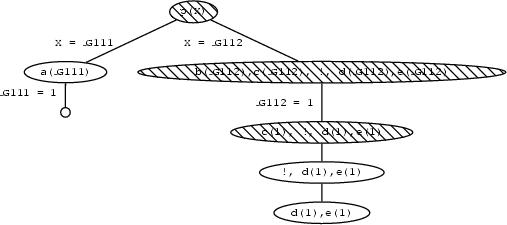
\includegraphics[scale = .95]{prologcutrace.jpeg}
\caption{Trace with cut (taken from \cite{website:cutprologunionedu})}
\label{fig:Trace with cut}
\end{figure}


\endnote{
  \david{say something about cut here}
\mehul{changed}
}

\section{Quasiquotation and \progLang{Haskell}}
\subsection{Quasiquotation}

When language is used to attribute properties to language or otherwise theorize about it, a linguistic device is needed that `turns 
language on itself'. Quotation is one such device \cite{website:quotationstanford}.

A metalinguistic device for referring to the form of an expression containing variables without referring to the symbols for those 
variables. Thus while ``not p'' refers to the expression consisting of the word not followed by the letter p, the quasi-quotation \newline
$\ulcorner$ not p $\urcorner$ refers to the form of any expression consisting of the word not followed by any value of the variable p 
\cite{website:quasiquotationfreedictionary}.

Quasi-quotation or Quine quotation is a linguistic device in formal languages that facilitates rigorous and terse formulation of general 
rules about linguistic expressions while properly observing the use--mention distinction \cite{wikiquasi}.

The use--mention distinction is a foundational concept of analytic philosophy,[1] according to which it is necessary to make a distinction 
between using a word (or phrase) and mentioning it \cite{website:usementiondistinctionwiki}.


\subsection{Quasiquotaion in \progLang{Haskell}}

Quasiquoting allows programmers to use custom, domain-specific syntax to construct fragments of their program. Along with 
\progLang{Haskell}'s existing support for domain specific languages, you are now free to use new syntactic forms for your EDSLs. Working 
with complex data types can impose a significant syntactic burden; extensive applications of nested data constructors are often required to 
build values of a given data type, or, worse yet, to pattern match against values. Allow \progLang{Haskell} expressions and patterns to be 
constructed using domain specific, programmer-defined concrete syntax \cite{haskellquasi, mainland2007s}.


\section{Meta syntactic variables}
Some sources for the topic 


\cite{website:metasyntacticvariableswiki}
A metasyntactic variable is a placeholder name used in computer science, a word without meaning intended to be
substituted by some objects pertaining to the context where it is used.
The word \markWord{foo} as used in IETF Requests for Comments is a good example.\endnote{%
  This regards
  \vspace*{-1.5\baselineskip}
  \begin{quote}\itshape
    A metasyntactic variable is a placeholder name used in computer science, a word without meaning intended to be
    substituted by some objects pertaining to the context where it is used. 
    The word \textsf{foo} as used in IETF Requests for Comments is a good example.
  \end{quote}
  \vspace*{-1.5\baselineskip}
  Some comments
  \begin{compactitem}
  \item
    ``IETF'' needs explanation.
  \item
    Because it is a something other than an English word with its ordinary meaning, ``foo'' needs to be marked
    up.
  \item
    The claim is overly broad.  In ``\texttt{\bfseries cat foo > bar}'', the word
    ``\texttt{\bfseries foo}'' is a file-name variable; it may be replaced by any file name
    (appropriately quoted for the surrounding shell).
    It is only when the variable ranges over syntax of an appropriate that the variable is metasyntactic.  For
    instance in ``\texttt{3 + 5 * }\textsf{term}'' the word ``\textsf{term}'' is a metasyntactic variable, the
    remainder is presumably either concrete or abstract syntax.
  \end{compactitem}
}

By mathematical analogy, a metasyntactic variable is a word that is a variable for other words, just as in algebra
letters are used as variables for numbers.
Any symbol or word which does not violate the syntactic rules of the language can be used as a metasyntactic
variable.




\cite{webiste:metasyntacticvariablescatb}
A name used in examples and understood to stand for whatever thing is under discussion, or any random member of a class of things under discussion. The word foo is the canonical example. To avoid confusion, hackers never (well, hardly ever) use `foo'\endnote{%
  This particular instance fixed.
  Avoid non-\textsc{ascii} characters.  Left single quote (u\(+\)x2018) should be entered in files as a grave
  accent (u\(+\)x60), and right single quote (u\(+\)x2019) as a plain single quote (0x27).

  Similarly, left double quote (u\(+\)x201c) should be entered as two grave accents, and right double quote as two
  single quotes.

  Em-dashes (u\(+\)x2014)---used to separate thoughts inside sentences---are typed as three minus signs.

  En-dashes (u\(+\)x2013), used to separate numbers, for instance 3--5, are typed as two minus signs.
}\elabel{non-ascii}
or other words like it as permanent names for anything. In filenames, a common convention is that any filename beginning with a metasyntactic-variable name is a scratch file that may be deleted at any time.

Metasyntactic variables are so called because they are variables in the metalanguage used to talk about programs
etc; they are variables whose values are often variables (as in usages like ``the value of f(foo,bar) is
the sum of foo and bar'').
However, it has been plausibly suggested that the real reason for the term ``metasyntactic
variable'' is that it sounds good.
To some extent, the list of one's preferred metasyntactic variables is a cultural signature.
They occur both in series (used for related groups of variables or objects) and as singletons.
Here are a few common signatures:


\cite{webiste:metasyntacticvariableswhatistectarget}
In programming, a metasyntactic (which derives from meta and syntax ) variable is a variable (a changeable value) that is used to temporarily represent a function . Examples of metasyntactic variables include (but are by no means limited to) ack, bar , baz, blarg, wibble, foo , fum, and qux. Metasyntactic variables are sometimes used in developing a conceptual version of a program or examples of programming code written for illustrative purposes.

Any filename beginning with a metasyntactic variable denotes a scratch file. This means the file can be deleted at any time without affecting the program.



\cite{webste:metasyntacticvariablesc2wiki}

A word, used in conversation or text that is meant as a variable. There is a fairly standard set in the ComputerScience\endnote{%
  ``ComputerScience'' should be ``Computer Science''.
}
culture. People tend to create their own if they are not exposed to others, which can be confusing. Of course, if you haven't seen them before they can be quite confusing. They are, however, useful enough that this is not enough reason to give them up.
Standard set: foo, bar, baz, foobar/quux, quuux, quuuux, ....

example: ``Suppose I have a list, foo, with a node, bar, ...''


\section{Chapter Recapitulation}


\end{document}
